
\chapter{Implementácia}



\section{Databáza zbraní}

\subsection{Augmentacia obrazkov}
- ktore triedy som implementoval


\section{Trénovanie klasifikátorov}
- rozdelenie dat do 3 skupin - trenovanie data, validacne, testovacie

\section{Zrhnutie kapitoly}

\begin{comment}

    \subsection{implementacia a vysledky- poznamky}
    \begin{enumerate}
        \item[$\bullet$] Z kade som realne cerpal data nakoniec
        \item[$\bullet$] Ako prebiehala augmentacia dat, opisat funkcie ktore sa pouzivaju pre dogenerovanie obrazkov a nazov tried ktore to implementuju.
        \item[$\bullet$] Obrazok trenovanie neuronovej siete
        \item[$\bullet$] Dosiahnute vysledky
        \item[$\bullet$] vytvorit velku prehladnu tabulku pre budu kompletne vysledky, tak ako to je na git-e opisane
    \end{enumerate}

\end{comment}

\subsection{Hodnotenie presnosti siete}

\begin{comment}

    \begin{figure}[H]
        \centering
        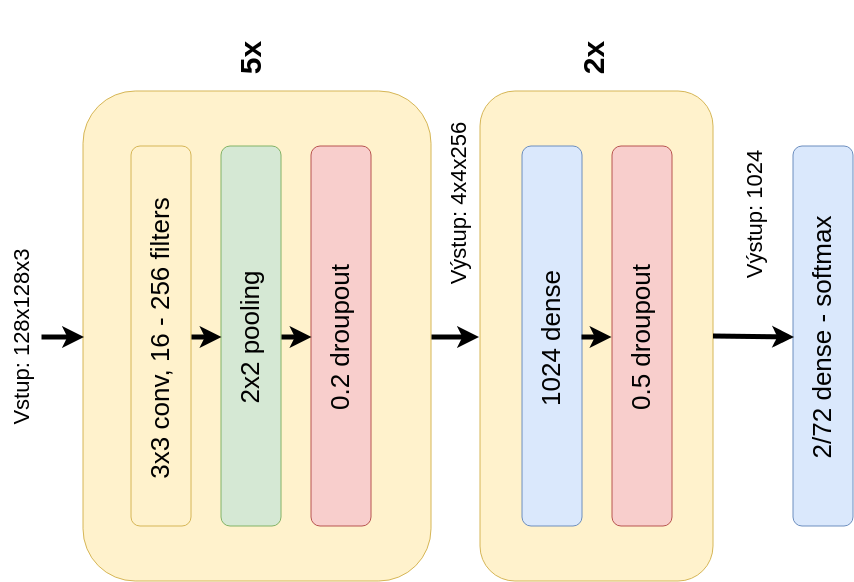
\includegraphics[width=0.32\textwidth]{AlexNet_Like}
        \caption{.}
        \label{pic:kNN}
    \end{figure}

    - Pridat ake optimalizatory a celkovo s akymi argumetmi spustat trenovanie, kolko epoch a pod...
    - Zdovodnovat preco prave taketo nastavenie konvolucnej siete.
    - pocet epoch bude potrebne zistit experimentalnych sposobom, alebo pouzit funkciu na save best of Keras-u

\end{comment}
